\section{Representation sensitivity beyond aggregate accuracy}
\subsection{Candidate order exposes hidden instability}
Figure~\ref{fig:order} juxtaposes prediction flips and the opposing correctness transitions hidden by their net accuracy change. Across the four historical local systems and four control tasks, reversal flips range from \ReversalMin\% to \ReversalMax\%; same-order repeats range from zero to \RepeatMax\%. These measurements support a presentation-sensitivity finding, rather than a uniform accuracy penalty.

\begin{table}[t]
\centering\small
\begin{tabular}{llrrr}
\toprule
Source & Model & Repeat flips & Reversal flips & $\Delta$ accuracy \\
\midrule
banking77 & Laya EN & 0.0 & 48.0 & +9.0 \\
banking77 & Laya Multi & 0.0 & 38.0 & +0.0 \\
banking77 & Llama & 4.0 & 65.0 & -25.0 \\
banking77 & Qwen & 1.0 & 39.0 & -18.0 \\
banking77 & Jev & 1.0 & 3.0 & +1.0 \\
massive\_en & Laya EN & 0.0 & 50.0 & -2.0 \\
massive\_en & Laya Multi & 0.0 & 46.0 & -7.0 \\
massive\_en & Llama & 5.0 & 51.0 & -2.0 \\
massive\_en & Qwen & 0.0 & 32.0 & -8.0 \\
massive\_en & Jev & 2.0 & 10.0 & -1.0 \\
\bottomrule
\end{tabular}

\caption{Matched candidate controls. Flip rates and accuracy differences are in percentage points. Reversal is compared with the same-order repeat; the repeat flip rate uses the corresponding original predictions. Source sizes differ and are shown in Figure~\ref{fig:order}.}
\label{tab:order}
\end{table}

Laya English on Banking77 illustrates the distinction: a 48\% flip rate accompanies a nine-point accuracy increase. Laya Multilingual flips 38\% of predictions with unchanged accuracy. Llama's 65\% reversal flips exceed its four-percent repeat flips, while its accuracy falls by 25 points. A mean accuracy change neither determines the number of affected decisions nor separates presentation effects from execution variation. Recording the paired transition structure is therefore an evaluation requirement whenever stability matters to the application.

\begin{figure}[p]
\centering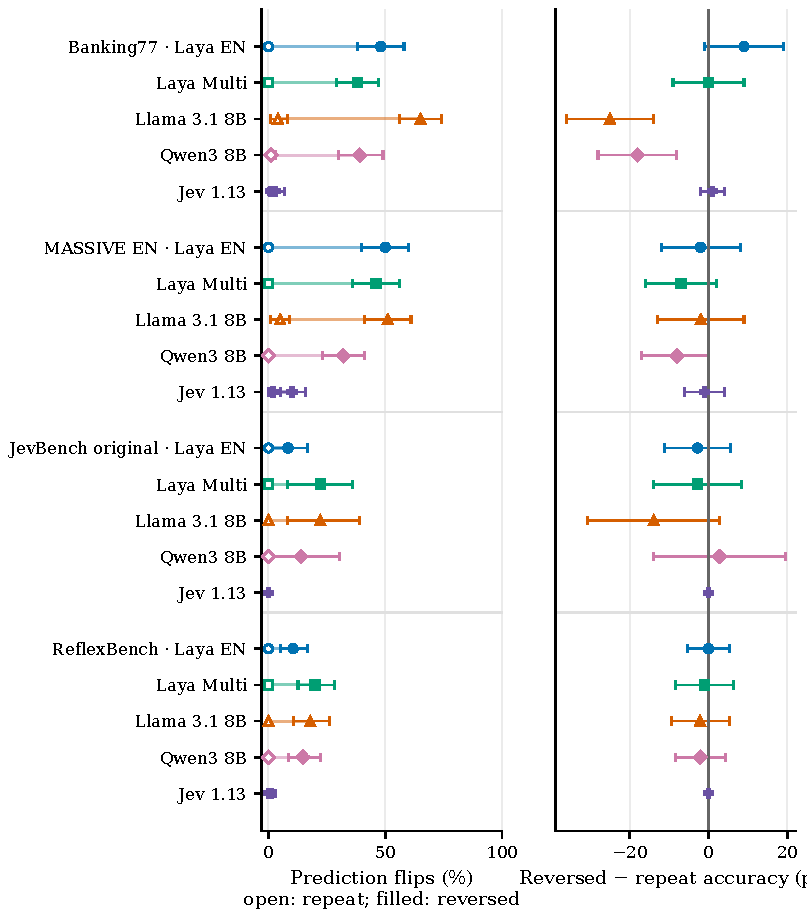
\includegraphics[width=.98\linewidth]{figures/fig_order.pdf}
\caption{Candidate presentation/code sensitivity. Left: bars show repeat-to-reversal regressions (correct to incorrect) and corrections (incorrect to correct), whose difference is the net accuracy effect. Right: open markers show original-to-repeat flips and filled markers repeat-to-reversal flips with pointwise 95\% paired cluster intervals. The control sets contain 100/100, 100/100, 36/18 and 95/95 decisions/source clusters respectively. Banking77 and MASSIVE use dataset references; JevBench and ReflexBench use authored or AI-reviewed references. No averaging across sources is performed.}
\label{fig:order}
\end{figure}

\subsection{Output encodings and language realizations}
The paired output-encoding effects depend on the task and system. On SST5, choice minus ordinal-score accuracy is \SSTEN, \SSTMulti, \SSTLlama\ and \SSTQwen\ percentage points for Laya English, Laya Multilingual, Llama and Qwen respectively. BoolQ effects are smaller and differ in direction. These are comparisons of complete interface encodings: instructions, candidate descriptions and adapter execution can all differ. They identify interface sensitivity, not the causal effect of a particular neural head.

The English/Chinese comparisons share source labels and sample identities. Chinese-minus-English accuracy is negative for every historical local system on both XNLI and MASSIVE under the existing English question wrappers. The magnitude varies substantially by model and source. Figure~\ref{fig:paired} places paired correctness effects beside prediction disagreement; a smaller average drop can still accompany many changed decisions. The practical implication is to validate the actual multilingual request rendering used by an application rather than transferring an English threshold or score by name.

\subsection{Context effects depend on the question}
Figure~\ref{fig:context} separates the choice and binary questions attached to each needle state. This split changes the interpretation of a pooled retrieval score. Llama retains strong choice retrieval across many lengths and positions while its binary damage question degrades with longer contexts. Laya English exhibits sharply different choice behavior when the relevant content appears at the start rather than the middle or end. Qwen's curves are comparatively stable in this fixed diagnostic. These patterns argue for a length-by-position-by-question analysis rather than a single context-window number or an assumed monotonic degradation law.

\subsection{Fresh policy interventions and codebook controls}
Table~\ref{tab:fresh} reports the original-state accuracies and joint original/counterfactual action success. The fresh diagnostic covers 96 base states per family, with eight matched variants. Figure~\ref{fig:confirmation} retains all six predeclared effects per model and policy, with simultaneous intervals within each six-effect family. The codebook experiment separates display order from answer-code identity for the two LLM adapters.
\begin{table}[t]
\centering\small
\begin{tabular}{llrrrrr}
\toprule
Policy & Model & Action & Review & Severity & Majority & Joint \\
\midrule
Access & Laya EN & 34.4 & 44.8 & 43.8 & 34.4 & 2.1 \\
Access & Laya Multi & 29.2 & 40.6 & 29.2 & 34.4 & 0.0 \\
Access & Llama 8B & 34.4 & 40.6 & 68.8 & 34.4 & 0.0 \\
Access & Qwen 8B & 66.7 & 53.1 & 79.2 & 34.4 & 46.9 \\
Access & Jev 1.13 & 100.0 & 89.6 & 95.8 & 34.4 & 100.0 \\
Refund & Laya EN & 25.0 & 77.1 & 31.2 & 25.0 & 0.0 \\
Refund & Laya Multi & 25.0 & 74.0 & 31.2 & 25.0 & 0.0 \\
Refund & Llama 8B & 33.3 & 74.0 & 59.4 & 25.0 & 0.0 \\
Refund & Qwen 8B & 25.0 & 74.0 & 43.8 & 25.0 & 1.0 \\
Refund & Jev 1.13 & 100.0 & 100.0 & 100.0 & 25.0 & 100.0 \\
Routing & Laya EN & 71.9 & 69.8 & 35.4 & 25.0 & 28.1 \\
Routing & Laya Multi & 24.0 & 63.5 & 33.3 & 25.0 & 0.0 \\
Routing & Llama 8B & 25.0 & 63.5 & 59.4 & 25.0 & 0.0 \\
Routing & Qwen 8B & 49.0 & 64.6 & 79.2 & 25.0 & 28.1 \\
Routing & Jev 1.13 & 54.2 & 100.0 & 95.8 & 25.0 & 29.2 \\
\bottomrule
\end{tabular}
\caption{Fresh policy reference accuracy (percent). Joint requires both original and one-field-counterfactual actions to be correct. Majority is the original action-label baseline. All rows have 96 paired base clusters; the complete machine-readable analysis includes pointwise cluster intervals and all reference-label distributions.}
\label{tab:fresh}
\end{table}


The fresh results separate invariance from supplied-rule competence. Jev achieves 100\% original and joint action success on refund and access policies, but only 54.2\% original and 29.2\% joint success on routing. Small reversal effects on that policy therefore do not establish correct rule application. Several local model/policy cells are near the action-majority baseline; low intervention effects in such cells can reflect consistently wrong decisions. We report base accuracy and joint counterfactual success alongside every stability diagnostic to expose this ambiguity.

Representation effects also depend on the supplied policy. Jev's authored Chinese routing rendering increases action accuracy by 45.8 percentage points, with a within-family simultaneous interval of [31.4, 60.2]; the underlying English facts and label IDs remain fixed. This is a difference between two complete policy/question/criteria renderings, not a general Chinese-language advantage. Laya English routing loses 46.9 points under explicitly irrelevant archived records. The full effect family, including null and opposite-direction results, appears in Figure~\ref{fig:confirmation}.

A post-hoc routing inspection localizes all 44 Jev English action errors to states where exactly one of \texttt{outage} and \texttt{paying} is true: every such state is routed to urgent support, although the policy requires both. All 52 states with matching boolean values are correct. The Chinese rendering is correct on all four boolean combinations. This behavioral pattern motivated the held-out wording test below; it did not isolate the cause because the original language intervention changed multiple text fields together.

The LLM codebook control shows why ordinary candidate reversal can be misleading (Figure~\ref{fig:codebook}). For Llama access decisions, reversing display alone changes no predictions, changing only the label-to-code assignment changes 55.2\%, and changing both again changes none. On routing, the corresponding values are 0\%, 62.5\% and 3.1\%. These are observed non-additive effects within the fixed adapter: apparent stability under the combined intervention can coexist with sensitivity to code identity. They do not identify an architectural mechanism. The codebook run is a separate inference block, so its repeat and both-change outcomes are not assumed identical to the earlier batch context.

\begin{figure}[t]
\centering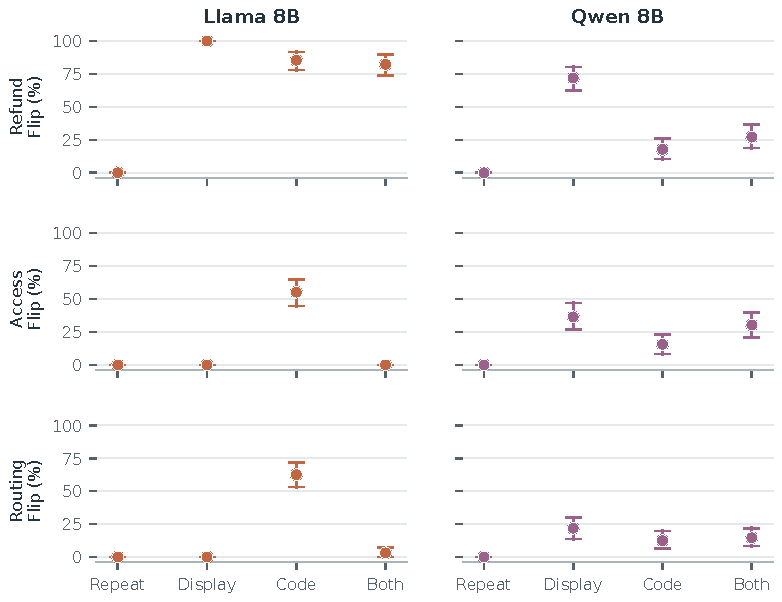
\includegraphics[width=.98\linewidth]{figures/fig_codebook.pdf}
\caption{Fresh LLM codebook controls: 96 base action decisions per policy and model, with pointwise 95\% paired cluster intervals. Display reverses semantic option order with code identity fixed; Code reverses code identity with semantic order fixed; Both changes both. Ground truth is an executable supplied policy. The code-only sensitivity can be hidden by the combined reversal.}
\label{fig:codebook}
\end{figure}

\subsection{Held-out wording: a proposed explanation fails to generalize}
The new routing cases balance all four outage/payment truth combinations by construction. Figure~\ref{fig:wording} reports the explicit-minus-compact wording effect on the 48 exclusive-or states, where erroneously interpreting ``or'' for ``and'' changes the action. Jev improves from 7/48 to 13/48 in English (+12.5 percentage points; paired 95\% CI [2.1, 25.0]), but falls from 46/48 to 13/48 in Chinese ($-68.8$ points; CI [$-81.3$, $-56.3$]). The explicit conjunction is therefore not a language-independent repair. Qwen improves by 29.2 points in English and 52.1 in Chinese, while Laya English worsens by 31.2 and 12.5 points respectively. We report these mixed results because a universal ``clearer wording helps'' account would be contradicted by the held-out data. The experiment changes one authored policy clause within each language; it does not identify whether the cross-language difference arises from translation quality, tokenization or model training.

\begin{figure}[t]
\centering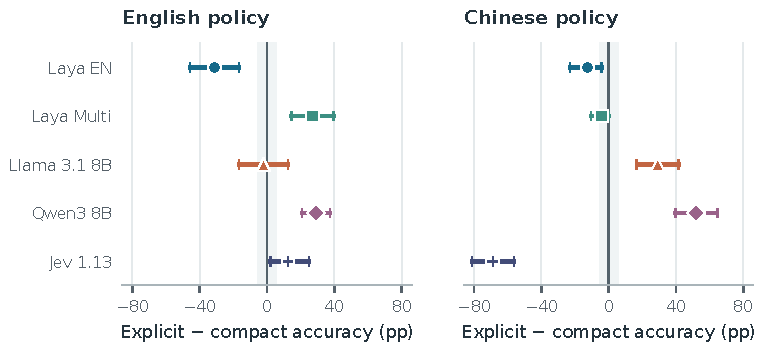
\includegraphics[width=.96\linewidth]{figures/fig_wording.pdf}
\caption{Held-out routing wording challenge on 96 new base states (48 XOR cases). Points are paired explicit-minus-compact action-accuracy effects; whiskers are pointwise 95\% bootstrap intervals stratified by generator seed and truth cell. Within each language only the first policy clause changes. English is the predeclared primary contrast; Chinese is secondary. The shaded band marks a $\pm5$-point descriptive region, not a significance threshold.}
\label{fig:wording}
\end{figure}
